\chapter{Marco teórico}
\label{marco}

Desde tiempos inmemorables las imágenes han acompañado al ser humano, desde las
pinturas rupestres en la Cueva de Altamira, pasando por los códices Mayas, los
daguerrotipos, las cámaras \textit{Pinhole} o los rayos X de Röntgen hasta las
imágenes del Curiosity Rover de la NASA. En este capítulo se introducen
conceptos básicos sobre las imágenes digitales, su procesamiento y su utilidad
en la lucha contra el cáncer de mama, al final del capítulo se hace un estudio
de trabajos similares.

\section{Breve introducción a las imágenes digitales}

% Pero ¿cómo una escena se convierte en un arreglo de píxeles?

Hay muchos tipos de imágenes digitales, en esta tesis nos enfocaremos en las
mamografías. Las imágenes digitales están formadas por una unidad básica
llamada \textit{pixel}. Una computadora representa una imagen como un arreglo
bidimensional de píxeles, cada posición de ese arreglo almacena valores
numéricos. Con el fin de conocer la posición de un pixel las imágenes tienen un
\textit{sistema de coordenadas}. A diferencia del sistema cartesiano, el origen
está en la parte superior izquierda (Figura~\ref{fig:coordinates}). 

\shorthandoff{>} % hack to combine tikZ and Spanish
    % TikZ picture with origin upper left
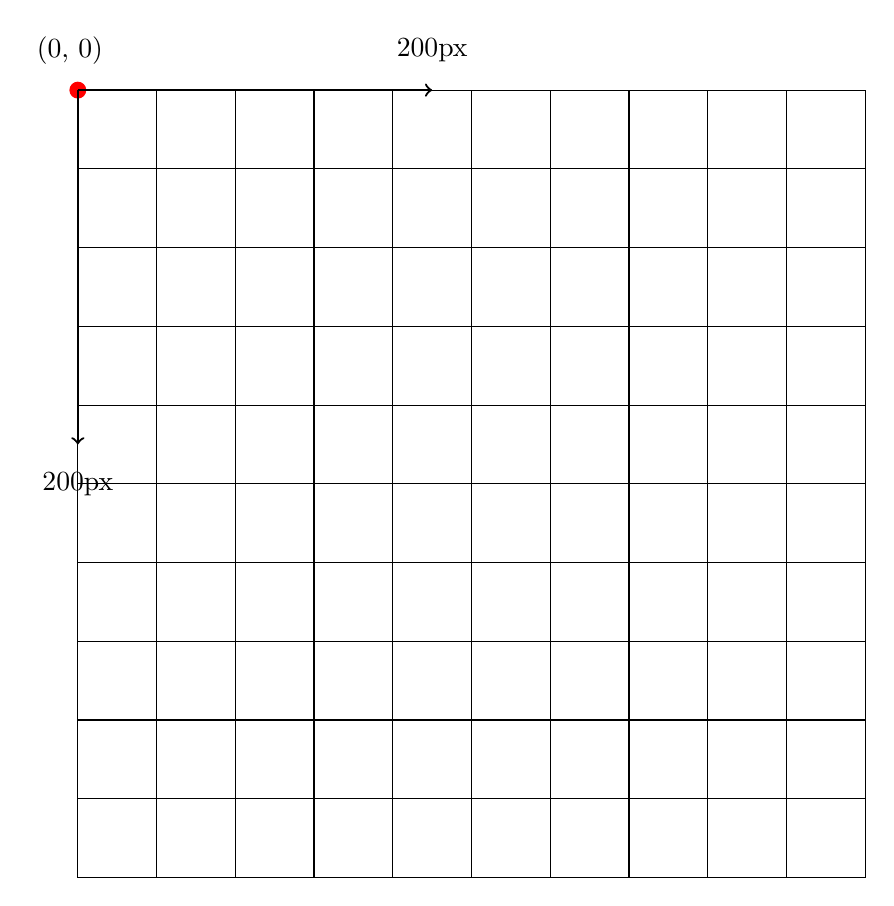
\begin{tikzpicture}[yscale=-1] 
    % 10x10 grid
    \draw (0, 0) grid (10, 10);
    % origin point
    \draw [color=red, fill=red] (0, 0) circle (0.1);
    % x-axis
    \draw [thick,->] (0, 0) -- (4.5, 0);
    % y-axis
    \draw [thick,->] (0, 0) -- (0, 4.5);
    % origin label
    \node at (-0.1, -0.5) {(0, 0)};
    % x-axis label
    \node at (4.5, -0.5) {200px};
    % y-axis label
\node at (0, 5) {200px};
\end{tikzpicture}

\shorthandon{>} 

% Improve explanation about light and discrete values 
La \textit{adquisición de imágenes} es el proceso por el cual una escena se
convierte en un arreglo de píxeles. El primer paso de este proceso se conoce
como \textit{muestreo} y consiste en la conversión de una distribución continua
de luz a su representación discreta. El segundo paso es la
\textit{cuantificación}, que consiste en la conversión a una escala de enteros.
De acuerdo a lo anterior, una imagen también puede definirse como una función
discreta como se muestra en la Ecuación~\ref{eq:discretized}. 

\begin{equation}
\label{eq:discretized}
    \begin{split}
            f(x,y) & = 
            \begin{pmatrix}
                f(1,1) & f(1,2) & \cdots & f(1,y) \\
                f(2,1) & f(2,2) & \cdots & f(2,y) \\
                \vdots & \vdots & \ddots & \vdots \\
                f(x,1) & f(x,2) & \cdots & f(x,y) \\
            \end{pmatrix}
    \end{split}
\end{equation}

\begin{table}
  \caption[Escala de grises]{Escalas de grises~\cite{burger2008digital}} 
  \label{table:grayscales}
\begin{center}
{\scriptsize
    \rowcolors{1}{}{lightgray} 
    \begin{tabular}{c|c|c}
    \hline
    {\bf Bits por pixel} & 
    {\bf Rango} & 
    {\bf Uso} \\
    \hline
    1  & 0\dots1     & Imágenes binarias: documentos, fax \\
    8  & 0\dots255   & Universal: Fotos, escaneos, impresiones   \\
    12 & 0\dots4095  & Alta calidad: Fotos, escaneos, impresiones   \\
    14 & 0\dots16383 & Profesional: Fotos, escaneos, impresiones   \\
    16 & 0\dots65535 & Altísima calidad: Medicina, astronomía   \\
    \hline
    \end{tabular}
}
\end{center}
\end{table}

En las imágenes \textit{a color} cada pixel generalmente tiene tres canales, es
decir, cada pixel almacena una tripleta de valores, las imágenes \textit{en
escala de grises} en cambio tienen un sólo canal por pixel. El rango de valores
que puede tomar cada pixel es conocido como \textit{bit de profundidad}. Cada
pixel puede almacenar $2^k$ valores diferentes que son números enteros en el
rango: $[0\dots2^k - 1]$ donde $0$ representa el color negro y $2^k$ el color
blanco. La Tabla~\ref{table:grayscales} sumariza información sobre las imágenes
en escala de grises y en la Figura~\ref{grayscales} podemos ver la misma imagen
con diferentes niveles de grises.

\begin{figure}[h]
    \centering

    \subfloat[16 niveles de grises]{\includegraphics[height=36mm]{images/lenna/lenna16.jpg}}
    \subfloat[8 niveles de grises]{\includegraphics[height=36mm]{images/lenna/lenna8.jpg}}
    \subfloat[4 niveles de grises]{\includegraphics[height=36mm]{images/lenna/lenna4.jpg}}
    \subfloat[2 niveles de grises]{\includegraphics[height=36mm]{images/lenna/lenna2.jpg}}

  \caption[Niveles de grises]{Imagen visualizada con distintos niveles de grieses. 
  (Imagen de Lenna obtenida de \cite{sipi})}
  
  \label{grayscales}
\end{figure}

Otros término básico para entender las imágenes digitales es la
\textit{resolución}, que sirve para especificar las dimensiones espaciales de
una imagen en el mundo real y es obtenida por el número de elementos de la
imagen por medida; por ejemlo, \textit{puntos por pixel}, (dpi, por sus siglas
en inglés). En la Figura~\ref{resolution} podemos ver la misma imagen con
diferente resolución.

\begin{figure}[h]
    \centering

    \subfloat[50 dpi]{\includegraphics[height=36mm]{images/dpi/dpi50.jpg}}
    \subfloat[25 dpi]{\includegraphics[height=36mm]{images/dpi/dpi25.jpg}}
    \subfloat[10 dpi]{\includegraphics[height=36mm]{images/dpi/dpi10.jpg}}
    \subfloat[5 dpi]{\includegraphics[height=36mm]{images/dpi/dpi5.jpg}}

  \caption[Resolución]{Diferentes resoluciones. Imagen visualizada con
  distintos valores \textit{dpi}. (Imagen de Lenna obtenida de \cite{sipi})}
  
  \label{resolution}
\end{figure}

El \textit{procesamiento de imágenes} es el conjunto de técnicas y algoritmos
utilizados con un propósito doble: mejorar la apariencia visual de las imágenes
al observador humano y preparar las imágenes para la medición de sus
estructuras y características.

Un \textit{histograma} es una distribución de frecuencia, el histograma de una
imagen describe la frecuencia y la intensidad de valores de una imagen
\cite{burger2008digital}. Los histogramas son herramientas valiosas para
examinar el contraste de una imagen. En la Figura~\ref{fig:histograms} se puede
ver la misma imagen con diferente contraste, se puede constatar que el
histograma está estrechamente relacionado con su contraste. La modificación de
histogramas es una tarea básica en el procesamiento de imágenes.

\begin{figure}[h]
    \centering

    \subfloat[Contraste normal\label{hist:b}]{\includegraphics[height=36mm]{images/histo/mandril.jpg}}
    \subfloat[Contraste óptimo\label{hist:d}]{\includegraphics[height=36mm]{images/histo/completerange.jpg}}
    \subfloat[Bajo contraste\label{hist:a}]{\includegraphics[height=36mm]{images/histo/rightskewed.jpg}}
    \subfloat[Alto contraste\label{hist:c}]{\includegraphics[height=36mm]{images/histo/leftskewed.jpg}}

    \bigskip

    \subfloat[Histograma de \protect\subref{hist:a}]{\includegraphics[height=36mm]{images/histo/histogram-right.jpg}}
    \subfloat[Histograma de \protect\subref{hist:c}]{\includegraphics[height=36mm]{images/histo/histogram-left.jpg}}

    \bigskip

    \subfloat[Histograma de \protect\subref{hist:b}]{\includegraphics[height=36mm]{images/histo/histogram-mandril.jpg}}
    \subfloat[Histograma de \protect\subref{hist:d}]{\includegraphics[height=36mm]{images/histo/completerange-histo.jpg}}

  \caption[Histogramas y contraste]{Histogramas y contraste. En
  \protect\subref{hist:b} se visualiza la imagen original y en
  \protect\subref{hist:d} la misma imagen después de modificar su contraste. En
  \protect\subref{hist:a} se visualiza la imagen con un bajo nivel de contraste
  y en \protect\subref{hist:c} en cambio la imagen tiene un alto nivel de
  contraste. (Imagen del Babboo obtenida de \cite{sipi})}
  \label{fig:histograms} 
\end{figure}

Procesar una imagen implica modificar el valor de sus píxeles. En las
\textit{operaciones sobre el punto} el valor de cada nuevo pixel depende
exclusivamente de su valor previo. Las operaciones sobre el punto están muy
relacionadas con la modificación de histogramas. Técnicas como ecualización de
histogramas o especificación de histogramas son operaciones sobre el punto. Por
otra parte existen técnicas que ocupan más de un pixel de la imagen original
para calcular el valor de los nuevos píxeles, estas técnicas son conocidas como
\textit{filtros}.

\section{Imágenes médicas}

% cross-sectional -> cortes transversales
Uno de los usos más importantes de las imágenes digitales recae en la medicina,
existe una gran variedad de imágenes médicas. Podemos mencionar las
\textbf{tomografías computarizadas} que son imágenes del corte transversal de
alguna parte del cuerpo, son generadas con rayos X. Las \textbf{resonancias
magnéticas} son generadas a partir de la propiedades magnéticas de un tejido.
La teoría sobre la cual descansa la generación de imágenes de este tipos está
ligada a la teoría especial de la relatividad y la mecánica cuántica.

Los \textbf{ultrasonidos} son generados a partir de ondas acústicas, su uso no
es exclusivo de la medicina, también son usados en la sismología, el estudio de
grietas microscópicas o en el estudio del fondo del mar. Las imágenes generadas
por la \textbf{medicina nuclear} se valen del uso de isótopos radioactivos. Por
último tenemos las \textbf{radiografías} (las mamografías son radiografías)
\cite{suetens2009fundamentals}.

\begin{figure}[h]
    \centering

    \subfloat[Tomografía]{\includegraphics[height=36mm]{images/medical/ct.jpg}}
    \hspace{1cm}
    \subfloat[Resonancia magnética]{\includegraphics[height=36mm]{images/medical/mr.jpg}}
    \hspace{1cm}
    \subfloat[Radiografía]{\includegraphics[height=36mm]{images/medical/cr-dx.jpg}}

  \caption[Algunos tipos de imágenes médicas]{Algunos tipos de imágenes médicas
  (Obtenidas de \cite{ica})}
  
  \label{medicalimages}
\end{figure}

\subsection{Mamografías}

El \textit{cáncer de mama} es un padecimiento en el que se desarrollan células
malignas en los tejidos de la mama, estas se duplican cada 100-300 días, un
tumor de 1 cm ha realizado alrededor de treinta duplicaciones antes de alcanzar
este tamaño, lo que implica que el cáncer de mama tiene, como mínimo, unos
siete años de evolución. Tomando en cuenta lo anterior se entiende la
importancia de la detección prematura de esta enfermedad~\cite{mxcancer}.

Cada estudio mamográfico tiene dos proyecciones o vistas por cada mama. La
proyección craniocaudal derecha (R-CC) e izquierda (L-CC) y la proyección
mediolateral oblicua derecha (R-MLO) e izquierda (L-MLO). Estas cuatro
proyecciones se pueden ver en la Figura~\ref{fig:views}. Las proyecciones CC se
obtienen de arriba para abajo y las proyecciones MLO de afuera para adentro.

\begin{figure}[h]
    \centering

    \subfloat[LCC\label{lcc}]{\includegraphics[height=35mm]{images/views/lcc.jpg}}
    \hspace{1cm}
    \subfloat[RCC\label{rcc}]{\includegraphics[height=35mm]{images/views/rcc.jpg}}

    \bigskip

    \subfloat[LMLO\label{lmlo}]{\includegraphics[height=35mm]{images/views/lmlo.jpg}}
    \hspace{1cm}
    \subfloat[RMLO\label{rmlo}]{\includegraphics[height=35mm]{images/views/rmlo.jpg}}

  \caption[Proyecciones de un estudio mamográfico]{Proyecciones de un estudio
  mamográfico. En \protect\subref{lcc} y \protect\subref{rcc} se aprecian las
  proyecciones craneocaudal izquierda y derecha, en \protect\subref{lmlo} y
  \protect\subref{rmlo} se aprecian las proyecciones mediolateral oblicua
  izquierda y derecha.}
  
  \label{fig:views}
\end{figure}

Actualmente se utilizan dos tipos de mamografías: las analógicas, mejor
identificadas como \textit{placas} y las digitales\footnote{Las mamografías
analógicas son conocidas como \textit{Screen-Film Mammography} (SFM) y las
digitales como \textit{Full-Field Digital Mammography} (FFDM), el nombre de los
equipos utilizados para generar estas imágenes es homónimo.}. Las tradicionales
mamografías analógicas están siendo reemplazadas por las mamografías digitales.
El uso de estas últimas representa una mejora en el proceso de adquisición de
la imagen, su almacenamiento y visualización~\cite{pisano2000current}. 

Las mamografías son imágenes que se obtienen al exponer la mama a una dosis
leve de rayos X. Los mastógrafos disponen de un receptor que captura la
radiación atenuada y por medio de un proceso electrónico forman una imagen
digital. Obtener una imagen mamográfica es un desafío debido a que la mama está
constituida por tejidos similares entre sí y porque algunas de las lesiones
buscadas por el radiólogo que indicarían la presencia de un tumor son pequeñas
o similares al tejido normal~\cite{mxcancer}. 

\subsection{Estándar DICOM}

DICOM\footnote{Digital Imaging and COmmunication in Medicine} es el estándar en
las imágenes médicas digitales, fue desarrollado por el Colegio Americano de
Radiología (ACR\footnote{American College of Radiology}, por sus siglas en
inglés) en conjunto con la Asociación Nacional de Fabricantes Eléctricos
(NEMA\footnote{National Electrical Manufacturers Association}, por sus siglas
en inglés)~\cite{national1996digital}. DICOM opera la adquisición de la imagen,
su transferencia, almacenamiento y visualización. 

Los dispositivos extraíbles como los discos compactos organizan su contenido a
través de un archivo llamado DICOMDIR que juega el rol de una pequeña base de
datos de archivos DICOM o un índice de archivos DICOM, colocado en la raíz de
un dispositivo extraíble. DICOMDIR organiza todos los datos del directorio en 
cuatro niveles: el nivel Paciente contiene $n$ Estudios, que a su vez contienen
$n$ Series que contienen $n$ Imágenes~\cite{pianykh2011digital}.  

Los archivos DICOM contienen metainformación organizada en forma de etiquetas,
en la Tabla~\ref{dicom:tags} podemos ver algunas de las etiquetas principales
de un archivo DICOM. 

\begin{table}
  \caption[Etiquetas DICOM]{Algunas etiquetas DICOM} 
  \label{dicom:tags}
\begin{center}
{\scriptsize
    \rowcolors{1}{}{lightgray} 
    \begin{tabular}{c|c}
    \hline
    {\bf Etiqueta} & 
    {\bf Información} \\
    \hline
    (0010, 0010) & Nombre del paciente\\
    (0008, 0070) & Fabricante\\
    (0008, 1030) & Descripción del estudio\\
    (0028, 0010) & Filas\\
    (0028, 0011) & Columnas\\
    \hline
    \end{tabular}
}
\end{center}
\end{table}

\subsection{BIRADS}

Como ya se mencionó antes, el diagnóstico de las mastografías lo llevan a cabo
radiólogos, sin embargo, el tratamiento está a cargo de médicos especializados.
Para evitar confusiones que puedan influir en el tratamiento el ACR desarrolló
un léxico estandarizado llamado BIRADS\footnote{Breast Imaging Reporting and
Data System Atlas}~\cite{reston2003birads}, que provee la terminología básica
y un sistema de clasificación para los estudios mamográficos. En la Tabla
\ref{birads} podemos ver un resumen de las categorías de evaluación.

\begin{table}
  \caption[Categorías de evaluación BIRADS]{Categorías de evaluación BIRADS}
  \label{birads}
\begin{center}
{\scriptsize
    \rowcolors{1}{}{lightgray} 
    \begin{tabular}{c | >{\centering\arraybackslash}m{1.8in} |
    >{\centering\arraybackslash}m{1.8in} }
    \hline
    {\bf Categoría} & 
    {\bf Descripción} &
    {\bf Sugerencia} \\
    \hline
    0 & Necesita evaluación adicional y/o más mamografías para comparar&\\
    1 & Negativo&\\
    2 & Hallazgo(s) benigno(s)&\\
    3 & Hallazgo(s) benigno(s) probable(s). & Se sugiere un seguimiento corto\\
    4 & Anormalidades sospechosas. & Una biopsia debe ser considerada \\
    5 & Altamente sugestivo de malignidad. & Se deben tomar acciones apropiadas\\
    6 & Malignidad probada&\\
    \hline
    \end{tabular}
}
\end{center}
\end{table}

BIRADS también clasifica los tipos de lesiones, entre las lesiones descritas en
la cuarta edición de BIRADS tenemos las \textit{masas}, las
\textit{calcificaciones}, las \textit{microcalcificaciones}, las
\textit{asimetrías focales}, las \textit{asimetrías globales} y la
\textit{distorsión de la arquitectura}. 

Una masa es una estructura tridimensional usualmente visible en dos
proyecciones ortogonales. Las calcificaciones y microcalcificaciones son
depósitos de calcio. Las asimetrías y la distorsión de la arquitectura no son
masas.

\subsection{Sistemas CAD}

Un sistema CAD puede mejorar el desempeño de los radiólogos en la predicción
del cáncer de mama. Varios sistemas de este tipo han sido desarrollados por la
comunidad científica, para la detección de masas~\cite{bellotti2006completely}
o clusters de microcalcificaciones~\cite{yu2000cad}. Sin embargo, sigue siendo
un problema abierto, sobre todo con la aparición de bases de datos de
mamografías digitales.

Las etapas para la construcción de un sistema CAD generalmente son:
preprocesamiento, selección de regiones de interés (ROI\footnote{Regions of
Interest}), extracción de características y finalmente un algoritmo de
aprendizaje supervisado, ver la Figura~\ref{fig:cadflowchart}.

\shorthandoff{>} % hack to combine tikZ and Spanish
    
% -------------------------------------------------
% Set up a new layer for the debugging marks, and make sure it is on
% top

\pgfdeclarelayer{marx}
\pgfsetlayers{main,marx}
% A macro for marking coordinates (specific to the coordinate naming
% scheme used here). Swap the following 2 definitions to deactivate
% marks.
\providecommand{\cmark}[2][]{%
  \begin{pgfonlayer}{marx}
    \node [nmark] at (c#2#1) {#2};
  \end{pgfonlayer}{marx}
  } 
\providecommand{\cmark}[2][]{\relax} 
% -------------------------------------------------
\begin{figure}[h]
\begin{center}
\begin{tikzpicture}[%
    >=triangle 60,              % Nice arrows; your taste may be different
    start chain=going below,    % General flow is top-to-bottom
    node distance=6mm and 60mm, % Global setup of box spacing
    every join/.style={norm},   % Default linetype for connecting boxes
    ]

{\small\ttfamily\fontfamily{lmodern}\selectfont
% ------------------------------------------------- 
% A few box styles 
% <on chain> *and* <on grid> reduce the need for manual relative
% positioning of nodes
\tikzset{
  base/.style={draw, on chain, on grid, align=center, minimum height=4ex},
  proc/.style={base, rectangle, text width=8em},
  test/.style={base, diamond, aspect=2, text width=5em},
  term/.style={proc, rounded corners},
  % coord node style is used for placing corners of connecting lines
  coord/.style={coordinate, on chain, on grid, node distance=6mm and 25mm},
  % nmark node style is used for coordinate debugging marks
  nmark/.style={draw, cyan, circle, font={\sffamily\bfseries}},
  % -------------------------------------------------
  % Connector line styles for different parts of the diagram
  norm/.style={->, draw, blue},
  free/.style={->, draw, green},
  cong/.style={->, draw, red},
  it/.style={font={\small\itshape}}
}
% -------------------------------------------------
% Start by placing the nodes
% Use join to connect a node to the previous one a

\node [proc, fill=brown!30, ultra thick] (p1) {Preprocesamiento};
\node [proc, fill=blue!30, join] (p2) {Selección de regiones de interés};
\node [proc, fill=green!30, join] (p3) {Extracción de características};
\node [proc, fill=purple!30, join] (p4) {Aprendizaje supervisado};
}
\end{tikzpicture}
\end{center}
  \caption[Etapas para la construcción de un sistema CAD]
  {Etapas para la construcción de un sistema CAD \cite{bozek2009survey}} 
  \label{fig:cadflowchart} 
\end{figure}

\shorthandon{>} 

En este trabajo se aborda la primera etapa en la construcción de un sistema
CAD. El \textbf{preprocesamiento} es la etapa previa al procesamiento de
imágenes \textit{per se}, el principal objetivo de esta etapa es mejorar la
calidad de la imagen para que quede lista para su posterior procesamiento
\cite{ponraj2011survey}, también se utiliza para mejorar la visibilidad del
observador~\cite{rahmati2010new}. 

\section{Preprocesamiento de mamografías}
% Preprocessing related works
% You organize this section by idea, and not by author or by publication

Varios trabajos de investigación se han desarrollado sobre el preprocesamiento
de mamografías. En esta sección hacemos una revisión de varios enfoques,
algunos de los cuales se rescataron en este trabajo para crear un método híbrido.

El preprocesamiento de mamogramas engloba algunas tareas también válidas en
otro tipo de imágenes como reducción del área de trabajo, remoción de ruido o
mejora de contraste, no obstante, también existe el \textit{preprocesamiento
orientado a mamografías} que comprende tareas como orientación de la dirección
de la mama, la supresión del músculo pectoral o la detección del pezón.

% ========== [ reduce work area ] ==========
La \textit{reducción del área de trabajo} es una tarea sencilla cuyo propósito
es reducir la imagen al objeto de interés con el fin de aminorar el tiempo de
ejecución de otros métodos subsiguientes y también mejorar su eficiencia. Este
procedimiento es expuesto por~\cite{holguinpre} y~\cite{dehghani2011method}.

% ========== [ denoising ] ==========
En el proceso de adquisición de las imágenes es posible que obtengan algún tipo
de contaminación, conocida como ruido. Los orígenes de ese ruido pueden ser
errores de transmisión, sensores con mal funcionamiento, secciones de memoria
defectuosas, entre otras cosas. En consecuencia, la \textit{remoción de ruido}
es indispensable antes de analizar los datos de las imágenes
\cite{motwani2004survey}.

En las imágenes mamográficas existen cuatro tipos de ruido: cuántico,
electrónico fijo, señales secundarias y \textit{quanta} secundario
\cite{hashimoto2008practical}. El ruido cuántico es predominante en imágenes
mamográficas, se genera debido a los rayos X con fotones de baja intensidad.
Este tipo de ruido puede ser modelado por la distribución de Poisson. El ruido
electrónico puede ser modelado como ruido gaussiano o aditivo, como se puede
ver en la Ecuación~\ref{eq:gaussian}:

\begin{equation}
\label{eq:gaussian}
            g = u + n,
\end{equation}

\noindent donde $u$ es la imagen mamográfica contaminada con ruido cuántico y
$n$ es el ruido gaussiano incorporado a la imagen mamográfica $g$.

Dos Santos~\cite{dos2009mammography} propone un método de dos etapas para
reducir el ruido cuántico, utilizando la Transformada de \textit{Anscombe} para
transformar el ruido cuántico en ruido aditivo que es eliminado utilizando el
filtrado Wiener. Su método fue evaluado utilizando un sistema CAD. 

Naveed propone un método similar al anterior que en primera instancia detecta
el ruido y luego lo filtra~\cite{naveed2012quantum}. La detección se lleva a
cabo utilizando redes neuronales y para la remoción del ruido se utilizan tres
filtros, que son \textit{non local mean} (NLM), el filtrado adaptativo de Wiener
y un método basado en el filtro \textit{Frost}. La remoción busca preservar los
detalles. Este estudio propone la eliminación del ruido impulsivo y cuántico.
Se evalúa el método comparando la precisión de algoritmos de
\textit{clasificación} en presencia y ausencia de ruido.

% ========== [ contrast enhancement ]  ==========
Otra tarea común en el preprocesamiento de mamografías es el \textit{realce o
mejora de contraste}. La Ecualización de Histogramas (HE\footnote{Histogram
Equalization}) es una técnica muy socorrida para mejorar el contraste en las
imágenes digitales, se utiliza para redistribuir los niveles de grises en una
imagen, lo que da como resultado un ajuste de contraste.

En las imágenes mamográficas mejorar el contraste de regiones pequeñas es más
importante que mejorar el contraste de forma global~\cite{mohan2013modified}.
La Ecualización Adaptativa de Histogramas (AHE\footnote{Adaptive Histogram
Equalization}) a diferencia de HE calcula el histograma de varias regiones de
la imagen (\textit{histogramas locales}).

AHE tiene algunas desventajas, es lento y tiende a mejorar el ruido, por lo que
muchas variantes de AHE han sido propuestas~\cite{pizer1987adaptive}. La
variante más destacada es la técnica llamada Ecualización Adaptativa de
Histogramas con Contraste Limitado (CLAHE\footnote{Contrast-Limited Adaptive
Histogram Equalization}~\cite{zuiderveld1994contrast}). CLAHE ha sido
ampliamente utilizado para modificar el contraste de
mamografías~\cite{pisano1998contrast, maitra2012technique}.

Rahmati~\cite{rahmati2010new} y Mohan~\cite{mohan2013modified} proponen mejoras
a CLAHE. Según Rahmati CLAHE mejora linealmente el frente y el fondo de la
imagen, o sea, se incrementa la visibilidad de las masas pero simultáneamente
se crean intensidades engañosas en el fondo, lo que puede conducir a la
detección de falsos positivos.

% ========== [ removal of pectoral muscle] ==========
La \textit{remoción del músculo pectoral} en imágenes con proyección MLO es
otra tarea de preprocesamiento orientado a mamogramas. Maitra propone un método
de tres fases, la fase inicial es la mejora de contraste con el algoritmo
CLAHE, después se aisla el músculo pectoral de la región de interés y
finalmente se suprime utilizando el algoritmo \textit{seeding region growing}.
Su método pudo aislar el músculo pectoral en la mayoría de las imágenes de
miniMIAS, ver Figura~\ref{fig:muscle}.

\begin{figure}[h]
    \centering
    \subfloat[\label{muscle:a}]{\includegraphics[height=45mm]{images/muscle/originalmuscle.jpg}}
    \hspace{1cm}
    \subfloat[\label{muscle:b}]{\includegraphics[height=45mm]{images/muscle/muscleremotion.jpg}}
    \hspace{1cm}
    \subfloat[\label{muscle:c}]{\includegraphics[height=45mm]{images/muscle/closeupmuscle.jpg}}

  \caption[Remoción del músculo pectoral]
  {Remoción del músculo pectoral. En \protect\subref{muscle:a} se aprecia la
  mamografía original, \protect\subref{muscle:b} muestra la remoción del
  músculo y \protect\subref{muscle:c} es un acercamiento. (Imagen obtenida de
  ~\cite{maitra2012technique})} 

  \label{fig:muscle}
\end{figure}

Akram también propone la remoción del músculo pectoral además de etiquetas y
artefactos~\cite{akram2013preprocessing}. Su propuesta utiliza el método de
contorno activo. Por su parte Mirzaalian plantea un algoritmo para la
extracción del contorno de la mama y otro para la extracción del músculo
pectoral~\cite{mirzaalian2007pre}. Para extraer el contorno de la mama utiliza
en conjunto la ecualización de histogramas, una técnica de convolución con una
máscara, que sirve como un filtro de paso bajo, binarización y etiquetado.

% =========[ surveys ]===========

Ponraj~\cite{ponraj2011survey} y Pisano~\cite{pisano2000image} hacen estudios
extensivos varios algoritmos utilizados para modificar imágenes mamográficas.

\section{Bases de datos similares}

% Other databases
Existen múltiples bases de datos de mamografias, públicas o privadas,
utilizadas en estudios relacionados a la detección del cáncer de mama, el
propósito principal de la mayoría de ellas es constituirse como un recurso para
el desarrollo de sistemas CAD. En la Tabla~\ref{table:overviewdb} se resumen
las características de varias bases de datos.

\afterpage{
    \clearpage
\begin{landscape}
%\begin{sidewaystable}
\begin{table}[h]
  \caption{Algunas bases de datos de mamografías digitales} 
  \label{table:overviewdb}
\begin{center}
{\scriptsize
    \rowcolors{1}{}{lightgray} 
    \begin{tabular}
    {c| >{\centering\arraybackslash}m{1in} | >{\centering\arraybackslash}m{1in}|c| 
    >{\centering\arraybackslash}m{0.6in} | >{\centering\arraybackslash}m{0.6in}|c|
    >{\centering\arraybackslash}m{0.6in} |c}
    \hline

    {\bf Nombre} & 
    {\bf Número de casos} & 
    {\bf Número de imágenes} & 
    {\bf Proyecciones} & 
    {\bf Tipo de archivo} & 
    {\bf Lugar de origen} & 
    {\bf Año} &
    {\bf Modo de adquisición} & 
    {\bf BIRADS} \\
    \hline
    mini-MIAS & 161  & 322    & MLO       & PGM   & Reino Unido    & 1994 & yes & yes \\[3.1ex] 
    DDSM      & 2620 & 10480  & MLO \& CC & LJPEG & Estados Unidos & 1999 & yes & yes \\[3.1ex] 
    BancoWeb  & 320  & 1'400  & MLO \& CC & TIFF  & Brasil         & 1999 & yes & yes \\[3.1ex] 
    INbreast  & 115  & 410    & MLO \& CC & DICOM & Portugal       & 2012 & yes & yes \\[3.1ex] 
    MIDAS     & 100  & 600    & MLO       & DICOM & Brasil         & 2011 & yes & yes \\[3.1ex] 
    IRMA      & -    & 10'509 & MLO \& CC & LJPEG & Alemania       & 2008 & yes & yes \\[3.1ex] 
    MIRaCLe   & 196  & 10480  & MLO \& CC & LJPEG & Grecia         & 2009 & yes & yes \\[3.1ex] 
    GPCalma   & 967  & 3369   & MLO \& CC & DICOM & Italia         & 2002 & no  & yes \\[3.1ex] 
    AMDI      & 967  & 3369   & MLO \& CC & DICOM & Canadá         & 2002 & no  & yes \\[3.1ex] 
    \hline
    \end{tabular}
}
\end{center}
\end{table}
%\end{sidewaystable}
\end{landscape}
} % end of afterpage

La mayoría de las bases de datos que existen almacenan mamografías
digitalizadas (SFM). Aunque es el recurso más viejo y no tiene soporte
actualmente mini-MIAS\footnote{The Mammographic Image Analysis Society Digital
Mammogram Database} sigue siendo un recurso ampliamente
utilizado~\cite{sucklingmini}. DDSM\footnote{The Digital Database for Screening
Mammography} es la base de datos pública más grande y también la más
utilizada~\cite{heath2000digital}.

IRMA\footnote{Image Retrieval in Medical Applications} es la conjunción de
otras cuatro base de datos (incluyendo las dos anteriores) cuyo propósito es
unificar los criterios utilizados para clasificar las imágenes de acuerdo al
tipo de lesiones~\cite{irma}.

MIRaCLe\footnote{Mammography Image reading for Radiologists and Computers
Learning Database} es un repositorio creado para entrenar y evaluar radiólogos
y también algoritmos CAD~\cite{antoniou2009web}. De manera similar, la
Universidad de Calgary ha creado un banco de imágenes conocido como
AMDI\footnote{Indexed Atlas of Digital Mammograms}~\cite{suri2006recent} que
funciona como \textit{atlas} y ayuda a los radiólogos a encontrar casos
similares cuando la emisión de un diagnóstico se torna complicada. De este
mismo proyecto se ha desprendido un sistema educativo~\cite{guliato2009indiam}.

MIDAS\footnote{Mammographic Image Database for Automated Analysis} contiene
muestras digitales tomadas entre la población femenina de Brasil, de esta base
de datos destaca la inclusión de secuencias de datos genómicas de los pacientes
y su apertura a la colaboración externa~\cite{fernandes2012midas}. BancoWeb
otra base de datos brasileña creada por LAPIMO\footnote{Laboratório de Análise
e Processamento de Imagens Médicas e Odontológicas}~\cite{matheus2011online}.

GPCalma\footnote{Grid Platform for Computer Assisted Library for MAmmography}
es una base de datos distribuida~\cite{lauria2006gpcalma}. GPCalma tiene la
particularidad de ser un proyecto vigente a pesar de haber iniciado hace muchos
años.

INbreast es un proyecto reciente~\cite{moreira2012inbreast}. Esta colección
contiene sólo mamografías digitales. Los autores proveen un conjunto de
directrices para ser consideradas en la construcción de una base de datos de
mamografías.

% Otras bases de datos mencionadas en la literatura son Trueta, LLNL, Málaga, NDMA.

